\chapter{Reinforcement Learning Model}
\label{chap:RLModel}
\section{Introduction}
\label{sec:IntroRL}
In the last chapter I analyzed the task-related activity patterns of the more frequent assembly-pair types. Significant task related activity was tested with Friedman test in the stimulus presentation (CS+/-) interval, stimulus continued\footnote{The window right before the reward delivery time, or the expected reward time in False Alarm trials, or the hypothetical reward time in Correct Rejection trials.} (CS+/-$_{cont}$.) interval, and at reward\footnote{Or expected reward in False Alarm trials, or Hypothetical Reward in Correct Rejection trials.}.\\We found that the major part of SPN-DAN pairs was activated few hundred milliseconds after the stimulus onset.\\SPN-DAN assembly-pairs activation was broader than the FSN-DAN activation, it is worth to recall that the mean lag of FSN-DAN pairs was shorter than the mean lag of SPN-DAN pairs. Time scale and activation profiles suggested that those two pair types reflect different component of the prediction error coding. Thus SPN-DAN pairs are good candidates for the evaluation signal crucial for reward prediction and reward prediction error coding as defined in classical reinforcement learning models.\\On the other hand I observed that FSN-DAN pairs were early activated by the stimulus onset and/or they activated phasically at the time of reward. The early activation could corresponds the detection of the stimulus, namely the first component of reward prediction error signalling not directly involved in the learning.\\FSN-DAN were homogeneous in their conditioned stimuli early response, either rewarded or unrewarded, but extremely diversified in their activation in correspondence to different events including choice and motivational status.\\ %In False Alarm trials a good portion of FSN-DAN is depressed before and after the expected reward time. Such activity could reflect emotional feelings of the animal during the task, that could be only partially involved in the reward prediction error definition given by reinforcement learning model.\\
The analysis of the assembly-pairs activity patterns cannot capture the dynamics of task. The task was such that the animal had to assign and re-assign a value to the rewarded odor to be able to predict the reward. Only taking in account this dynamic I can understand whether and SPN-DAN specialize in the reward prediction error computing. Since FSN-DAN seemed not involved in reward prediction error coding, I used those assembly-pairs as control for the further analysis.\\To take this into account, I implemented reinforcement learning models (\cite{RescorlaWagner}, \cite{Sutton}, \cite{SuttonBarto}).\\$"$Reinforcement learning$"$ is an area in machine learning, in which an agent tries to learn the best action to take, depending on the circumstances in which this action will be performed, this approach can incorporate any changes in the environment of the decision making process. $"$Learning by reinforcement$"$ is derived from concepts in psychology where the agent receives a reward or punishment. Depending on the decision made, through the experience he is able to associate the actions that generate the greatest reward for each situation that the environment presents, and to avoid unrewarded actions or actions that generate punishment.\\Machine learning uses the same idea: the machine observes a state and, based on this, chooses an action to take and receives the reward associated with that specific action in that state, thus obtaining the information of this specific combination. The process is repeated until the machine is able to choose the best action to take for each of the possible scenarios to be observed in the future.\\
\section{Model}
\label{sec:Model}
%%%%%{\color{blue}Start writing equation of reinforcement learning}
%%%%%First Option I tried, Georgia's option {\color{red}cite Georgia's paper}
%%%%%We set up four RL models and I chose the one that better fitted the behaviour for the regression analysis.
Reinforcement learning model are usually set up as follows:
\begin{itemize}
    \item At each trial $t$ of the experiment, a state $s$ is observed, this is an input of the model.
    \item After the stimulus presentation, the animal has the chance to take an action, and according to the choice made, the reward is delivered. The reward is a vector $r(t)$, each vector component indicates the reward value delivered at the trial $t$, the reward vector is an input of the model.
    \item After the reward delivery, the animal computes the reward prediction error, that is evaluated in the model as the difference between the actual reward and the expected reward.
    \item States values are the expected reward values and they are updated according to the last expected values and the reward prediction error and it is modulated by the learning rate.
    \item The learning rate is often a constant free parameter, however it has been shown that a time dependent variable better describes the learning dynamic (\cite{Funamizu}, \cite{Daw}).
    \item Learned values are then translated into action probabilities via a softmax function, maximized with respect some free parameters.
\end{itemize}
In the presented reversal learning, two odor were presented and only one was associated with a reward with a probability of 0.9. Each time one odor was presented the mouse chose to take the action (lick or no-lick) that maximized the reward and minimized his effort. The task was considered learnt when the animal was able to lick for the rewarded odor and not lick when the unrewarded odor was presented. The performance criterion was set at $79\%$.\\To model this learning process, a Q Learning-Forgetting model (Q L-F model) starting from an hybrid Rescorla-Wagner model Pearce-Hall update mechanism (\cite{RescorlaWagner}, \cite{PearceHall}, \cite{Li}, \cite{Costa}, \cite{Koppe}) was implemented. The model contained an update of unchosen option using learning and forgetting parameters (\cite{ItoDoya1}, \cite{Katahira}).
The model assigns each state $s$ and action $a$, an action value $Q_{s,a}(t)$, where $t$ is the index of the trial. In the specific case I have two states, corresponding to the two odors presented and two possible actions, i.e., lick or no-lick. 
Based on the set of action values the model transforms the learned values into action probabilities via a softmax function to be maximized with respect to a set of parameters.\\The action value for the chosen option is updated by
\begin{equation}
Q_{s,a}(t+1)  = Q_{s,a}(t)+k_L\cdot\alpha_L(t)\cdot\delta(t), \hspace{0.3cm} with \hspace{0.3cm}\delta(t)=r(t)-Q_{s,a}(t-1)
\label{eq:Qlearning}
\end{equation}
where $\delta$ is the prediction error, i.e., the difference between the reward $r(t)$ and the expected reward value $Q_{s,a}(t)$ for an action $a$ given a state $s$, $k_L$ is the learning parameter and $\alpha_L(t)$ is the Pearce-Hall associability for the chosen option; this is a trial-dependent rate component which adjusts in accordance with the average accuracy of recent predictions, evolving by
\begin{equation}
   \alpha_L(t)=(1-\eta)\cdot\alpha(t-1)+\eta\cdot\abs{\delta(t)},\hspace{0.3cm} \eta\in[0,1]
    \label{eq:Alphalearning}
\end{equation}
Note that the $t$'s associability depends on absolute prediction errors from past trials, but not the current one, ensuring that $\delta(t)$ was not double counted in the value update.\\The associability term in eq. \ref{eq:Alphalearning} measures the attention of the animal to the cue, in other terms it is nothing but the uncertainty of the animal to get the reward. 
For the unchosen option $a'\neq a$ the action value is updated by
\begin{equation}
    Q_{s,a'}(t+1) = Q_{s,a'}(t)-k_F\cdot\alpha_F(t)\cdot Q_{s,a'}(t)
    \label{eq:Qforgetting}
\end{equation}
where $k_F$ is the forgetting rate (\cite{ItoDoya1}), in this model the associability for the unchosen option is as well a time-dependent component and evolves as follows
\begin{equation}
    \alpha_F(t)=(1-\eta)\cdot\alpha_F(t-1)+\eta\cdot Q_{s,a'}(t), \hspace{0.3cm}
    \eta\in[0,1]
    \label{eq:Alphaforgetting}
\end{equation}
Learned values are then translated into action probabilities via a softmax function:
\begin{equation}
p(a|s)=\frac{e^{\beta Q_{s,a}(t)}}{\sum_l e^{\beta Q_{s,l}(t)}}
\label{eq:ProbMod}
\end{equation}
where $\beta$ is a free parameter, usually called inverse temperature, that governs the animals$'$ exploitation/exploration.\\
Note that using $k_F = 0$ the model is reduced to the hybrid Rescorla Wagner model. I applied to the data four different version of the model, the one shown here as presentation is the one that best fit the behavioural data. The other three versions are:
\begin{description}
    \item[i.] \textbf{Hybrid Rescorla-Wagner (hRW).} The presented model is reduced to an hybrid Rescorla Wagner/Pearce Hall update mechanism when we use a learning parameter $k=k_L$, and no forgetting parameter, i.e. $k_F = 0$.
    Then, if $a$ represents the chosen option and $a'\neq a$ the unchosen option, the action values evolve as follows\\
    $\begin{array}{lcl}
    Q_{s,a}(t+1)&=& Q_{s,a}(t)+k\cdot\alpha(t)\cdot\delta(t), \hspace{0.3cm} with \hspace{0.3cm}\delta(t)=r(t)-q_{s,a}(t)\\
    Q_{s,a'}(t+1)&=&Q_{s,a'}(t)\\
    \end{array}$
    \item[ii.] \textbf{Rescorla-Wagner with two learning rate modulations $\kappa$ ($2\kappa$).} Let $a(t) \in \{1,0\}$ denote the option was chosen at trial $t$, where $1$ stands for "lick" and $0$ stands for "no-lick". I introduce then two learning parameters $k_{1}$ and $k_{0}$ respectively for the choice $a=1$ and $a=0$ to be estimated by the model, while $k_F$ is fixed to zero.
    Then when the choice $a=1$ is realized, the action values evolves by\\
   $\begin{array}{lcl}
       Q_{s,1}(t+1)&=&Q_{s,1}(t)+k_1\cdot\alpha(t)\cdot\delta(t)\\
         Q_{s,0}(t+1)&=&Q_{s,0}(t)\\ 
    \end{array}$\\
    while if the choice $a=0$ is realized I have\\
    $\begin{array}{lcl}
       Q_{s,0}(t+1)&=&Q_{s,0}(t)+k_0\cdot\alpha(t)\cdot\delta(t)\\
         Q_{s,1}(t+1)&=&Q_{s,1}(t)\\ 
    \end{array}$
    \item[iii.] \textbf{Rescorla-Wagner with two $\eta$ parameters ($2\eta$).} I use a learning model, without forgetting parameters, and I introduce two $\eta$ parameters $\eta_1$ and $\eta_0$ for the choice $1$ and $0$ respectively, to be estimated by model. The associability $\alpha$ evolves as follow:\\
   $\begin{array}{lcll}
    \alpha(t) & = & (1-\eta_1)\cdot\alpha(t-1)+\eta_1\cdot\abs{\delta(t)} & \mbox{if\,\,}  a=1,\\
    \alpha(t) & = & (1-\eta_0)\cdot\alpha(t-1)+\eta_0\cdot\abs{\delta(t)} & \mbox{if\,\,}  a=0.\\
    \end{array}$\\
    and action values for the chosen option evolving consequently as in the equation \ref{eq:Qlearning}.
\end{description}
Figure \ref{fig:L-Fmodel} provides an example of animal performance and RL-models action values. When the odor was rewarded the expectancy of reward related to the lick action ($Q_{1,1}$ in original and $Q_{2,1}$ in reversal) reproduced the hit performance. 
\begin{figure}
    \centering
    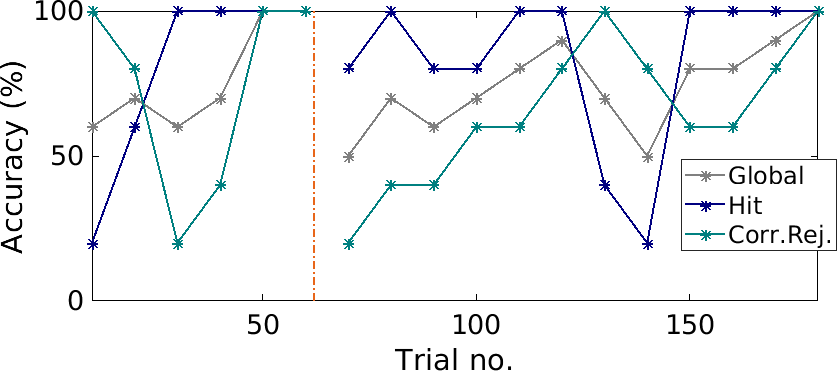
\includegraphics[scale=0.4]{figures/PerfEndrevAn1.png}
    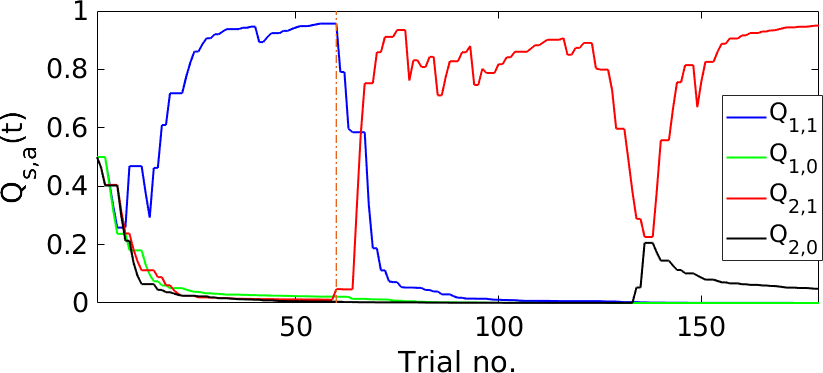
\includegraphics[scale=0.4]{figures/QValuesEndrevAn1.png}
    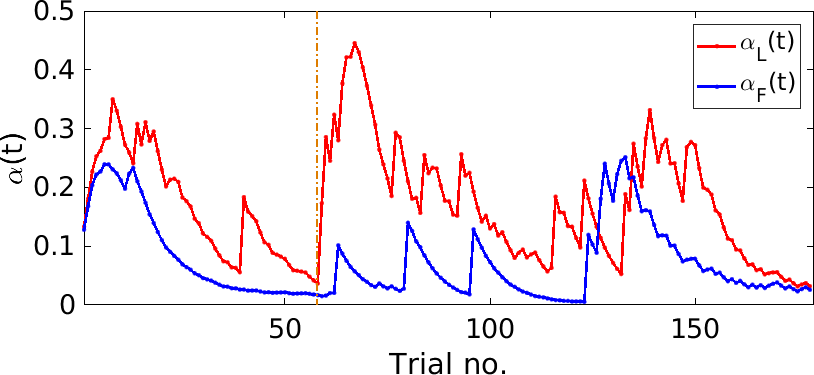
\includegraphics[scale=0.4]{figures/AlphaEndrevAn1.png}
    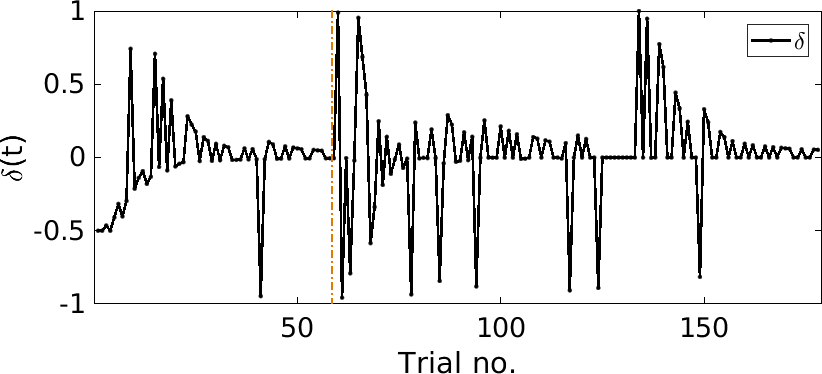
\includegraphics[scale=0.4]{figures/DeltaEndrevAn1.png}
    \caption{Example of animal performance and RL model action
values. Odor 1 was rewarded only in the original phase, while Odor 2 was rewarded only in the reversal phase. In order from top to bottom: Performance in all trials, in hit trials and correct rejection trials. RL model action values for the action lick, when odor 1/odor 2 occurs (blue/red) and the action no lick when odor 1/odor 2 is presented (green/black). Uncertainty $\alpha_L(t)$ for the chose option (red line), and $\alpha_F(t)$ for the unchosen option (blue line). Prediction error $\delta(t)$.}
    \label{fig:L-Fmodel}
\end{figure}
\section{Model Estimation and Selection}
\label{sec:Behavior}
We conducted a log-likelihood based model comparison analysis, that judged which model better reproduced the actions taken by the animals, given the states, the model values and the model parameters. Given the action probabilities as defined by equation \ref{eq:ProbMod}, the model log-likelihood can be expressed as $l=\sum_{t} \log p(a_t|s_t,Q_t,\theta_t)$. Where $\theta$ are the model parameters (defined model by model in the previous session), which were estimated for each animal by maximum likelihood using MATLAB$'$s active set algorithm (fmincon), which relies onsolving the Karush-Kuhn-Tucker equations by quasi-Newton methods, starting from 100 different initial conditions to avoid local minima\footnote{Part of the scripts used were adapted from some previous scripts developed and provided by Dr. Georgia Koppe}.\\The hybrid Rescorla-Wagner model (i.) has fewer parameters with respect to the three adapted Rescorla-Wagner versions proposed (ii.,iii., Q L-F model), and all the three versions can be transformed to the hybrid Rescorla-Wagner by imposing constraints on the former$'$s parameters. Thus, using Likelihood Ratio tests for nested models I could test for each alternative model proposed whether it was better than the hybrid Rescorla-Wagner. Likelihood ratio test (LRT) is formalized as the ratio of the likelihood functions of the models to compare (\cite{NeymanPearson}, \cite{King}) as follows:\\
 \hspace{5cm} $LRT = -2 \log (\frac{\mathcal{L}_s(\hat{\theta})}{\mathcal{L}_g(\hat{\theta})})$\\
where $\hat{\theta}$ are the parameters values that maximize the likelihood function.
The simpler model (s) has fewer parameters than the general model (g), the latter can be reduced to the simpler model after imposing some constraint (null hypothesis).\\LRT compares the fit of two models and has an asymptotic $\chi^2$ distribution. The null hypothesis is that the smaller model is the $"$best$"$ model and it is rejected when the test statistic is large. In other words, if the null hypothesis is rejected, then the larger model is a significant improvement over the smaller one. In this way, in each test I tested whether the addition of one parameter to the pure Rescorla-Wagner model was needed and brought a significant improvement. The tests were conducted separately for each animal.
\begin{table}[H]
\begin{tabular}{|p{2.5cm}|p{2.5cm}|p{2.5cm}|p{2.5cm}|}
\hline
\multicolumn{4}{|c|}{\cellcolor{blue!25}{Comparison between hRW model and Q L-F model (Likelihood ratio test)}}\\
\hline
 \cellcolor[gray]{0.9} animal & \cellcolor[gray]{0.9} $\mathcal{L}_s / \mathcal{L}_g$& \cellcolor[gray]{0.9} $\chi^2 statistic$ & \cellcolor[gray]{0.9} p-value\\
 \hline
 1& 1.77e-25 & 113.98 & \colorbox{cyan}{0}\\
 \hline
 2& 4.02e-08 & 34.05 & \colorbox{cyan}{5.35e-09}\\
 \hline
 3 & 1.34e-04 & 17.82 & \colorbox{cyan}{2.42e-05}\\
 \hline
 4 & 3.43e-34 & 154.10 & \colorbox{cyan}{0}\\
 \hline
 5 & 6.18e-19 & 83.85 & \colorbox{cyan}{0}\\
 \hline
 6 & 1.22e-08 & 36.44 & \colorbox{cyan}{1.57e-09}\\
 \hline
 7 & 1.62e-24 & 109.55 & \colorbox{cyan}{0}\\
 \hline
 8 & 3.77e-10 & 43.39 & \colorbox{cyan}{4.47e-11}\\
 \hline
 9 & 0.95 & 0.09 & \colorbox{yellow}{0.75}\\
 \hline
 10 & 2.87e-05 & 20.91 & \colorbox{cyan}{4.80e-06}\\
 \hline
 11 & 1.25e-38 & 174.53 & \colorbox{cyan}{0}\\
 \hline
 12 & 2.37e-05 & 21.30 & \colorbox{cyan}{3.93e-06}\\
 \hline
 13 & 8.16e-07 & 28.03 & \colorbox{cyan}{1.19e-07}\\
 \hline
 14 & 3.99e-02 & 6.44 & \colorbox{cyan}{1.11e-02}\\
 \hline
 15 & 7.37e-16 & 69.68 & \colorbox{cyan}{1.11e-16}\\
 \hline
 16 & 7.24e-43 & 194.06 & \colorbox{cyan}{0}\\
 \hline
 17 & 2.67e-05 & 21.06 & \colorbox{cyan}{4.45e-06}\\
 \hline
\end{tabular}
\caption{Likelihood ratio test performed in 17 animals. The null hypothesis is that the model with fewer parameters is the best model. In last column the p-value of the $\chi^2$ statistic, in blue p-values below significance level $\alpha_s=0.05$ indicate that the null hypothesis is rejected. In yellow not significant p-values. In the comparison between the hRW and the Q L-F model, Q L-F revealed to be the best model.}
\label{tab:ModelComparison}
\end{table}
In the comparison between the hybrid Rescorla-Wagner (hRW) and the learning-forgetting model (Q L-F), the latter Q L-F model revealed to be the $"$best$"$ model in $95\%$ of cases. The addition of the extra parameter in Q L-F improved the fit. In table \ref{tab:ModelComparison} LRT and the relatives $\chi^2$ statistic and p-values in two paradigms.\\
Q L-F and hRW were nested model, that allowed the use of LRT for comparison. To understand whether the Q L-F was the best model among the three adapted version of the hRW, a further test was needed . In this case, since the models were not nested, but had same number of parameters, the best model was evaluated using the Bayesian Information Criterion (BIC), that is a criterion for model selection among a finite set of models where the model with the lowest BIC is preferred (\cite{Schwarz}, \cite{NeathCavanaugh}). BIC is formally defined as 
\begin{equation*}
    BIC=k\log(n)-2\log(\hat{\mathcal{L}})
\end{equation*}
where: ${\hat{\mathcal{L}}}$ is the maximized value of the likelihood function of the model, $n$ is the sample size, $k$ is the number of parameters estimated by the model. Following Raftery$'$s approach (\cite{Raftery}), a difference of BIC lower than 2 between two models is barely worth mentioning, a difference between 2 and 5 is positive, a difference between 6 and 10 is strong, and a difference larger than 10 is very strong.\\The Bayesian Information Criterion (BIC) elected the learning-forgetting model as the best model (figure \ref{fig:BIC}).
\begin{figure}
    \centering
    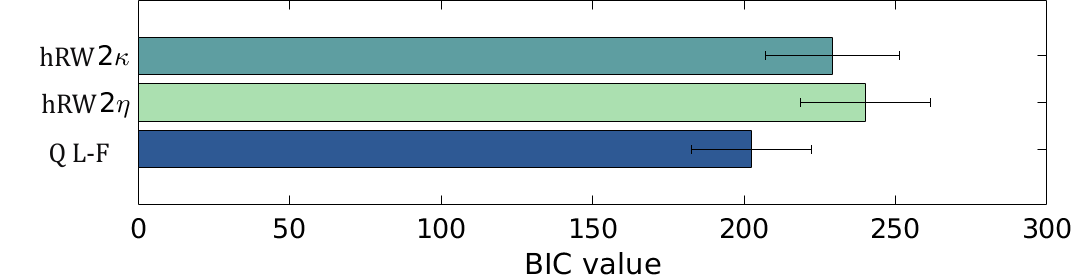
\includegraphics[scale=0.45]{figures/BIC_Value.png}
    
    \vspace{1cm}
    
    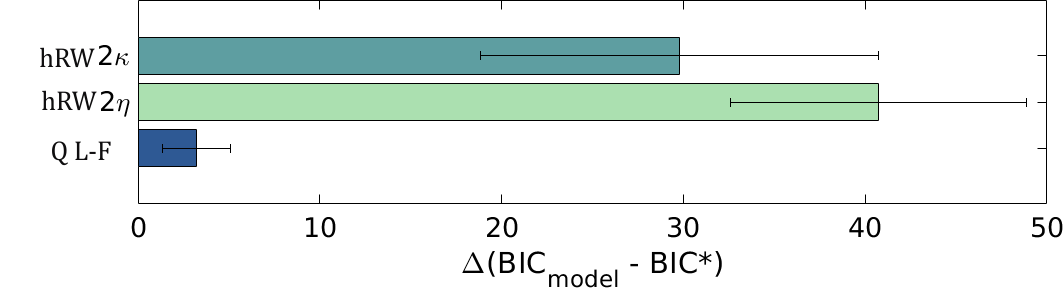
\includegraphics[scale=0.45]{figures/DeltaBIC.png}
    \caption{\textbf{Top:} BIC for the three models proposed as alternative of the hybrid Rescorla-Wagner. The BIC was computed separately for each animal, and mean and standard error were reported. The best model was the model with the lower BIC, indicated as BIC*. The Q L-F model revealed to be the best model for the more than 80$\%$ of the animals. The $2\eta$ model was never the best model and the $2\kappa$ model was the best model for less the 20$\%$ of the animals. It is worth to notice that also in cases when the Q L-F model was not the best model, the difference between its BIC and the BIC* rarely passed a value $>5$. \textbf{Bottom:} the difference between the BIC of each model (BIC$_{model}$) and BIC*, this difference was computed separately for each animal and mean and standard error were reported.}
    \label{fig:BIC}
\end{figure}
Figure \ref{fig:4models} displays action values of the four proposed models. In the gray box the animal's performance is reported as indication of actions taken in task. The importance of the forgetting term is particularly clear if I look at the action values $Q_{1,0}(t)$ in original phase and $Q_{2,0}(t)$ in reversal phase curves. The unchosen option (which often corresponded to no-lick for the unrewarded odor once that the task was learnt) did not update the action values in models devoid of the forgetting term (hRW, 2$\eta$, 2$\kappa$). This implied that the action value for the state-action combination of rewarded odor and no-lick action remained stable at the value of the last update when the no-lick action was chosen (see $Q_{1,0}$ in A.,B.,C.), until the no-lick was chosen again. This value however did not correspond to the real value assigned by animals persistently licking when that odor was presented; in such a task I could assume in fact that when an animal made a choice not only assigned a value to the current state according to that choice, but it also inferred the value of the current state for the unchosen option. The learning-forgetting model instead reproduced in this sense the entire perspective of learning dynamic, assuming that the unchosen option was consciously not taken at the moment that the opposite action was chosen. The small increases of $Q_{1,0}$ and $Q_{2,0}$ that occurred respectively before trial no. 50 and after trial no. 150 (figure \ref{fig:4models}) was due to the fact that when the animal was too reluctant to lick, a reward was given to encourage the lick choice for the rewarded odor. 
\begin{figure}
    \centering
    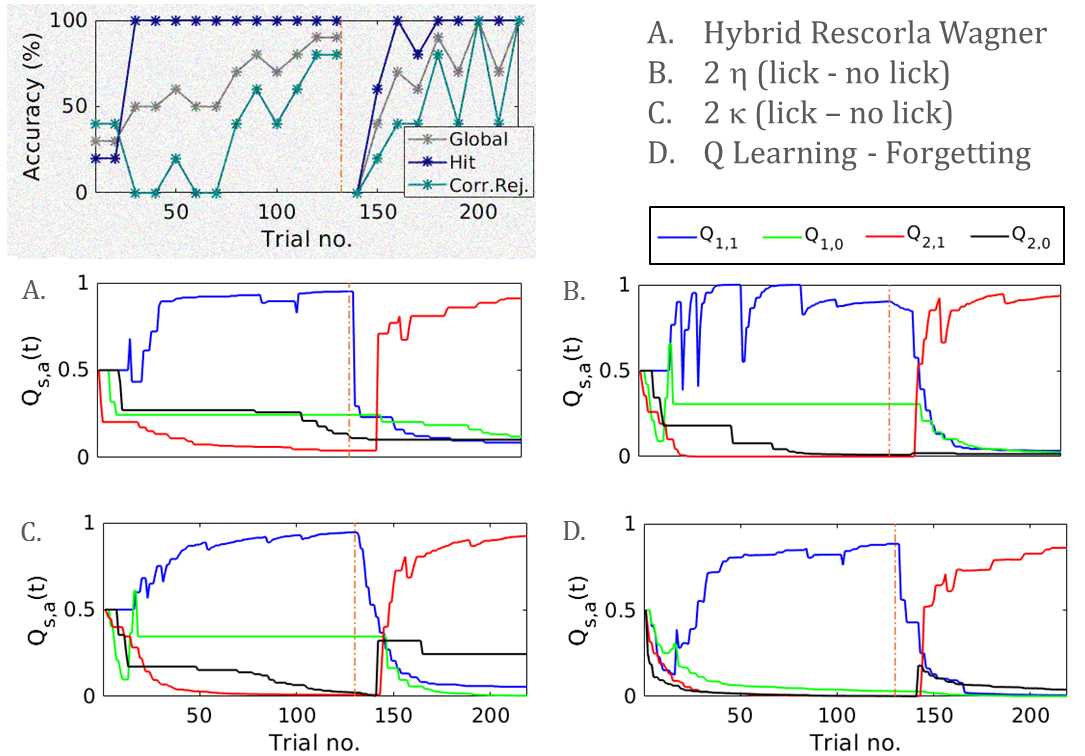
\includegraphics[scale=0.66]{figures/Resume4models3.png}
    \caption{Animal performance (top left) compared to the action values of the four models (A.B.C.D.)}
    \label{fig:4models}
\end{figure}
\section{Uncertainty and prediction error signal\\in assembly-pair types}
\label{sec:CorrRL}
VS-VTA interactions are assumed to be able to predict the reward and compute the prediction error. I used a reinforcement learning model to parameterize the learning functions. If the assembly-pairs code for some aspects of the learning, they will correlate with some specific reinforcement learning functions.
\begin{figure}
    \centering
    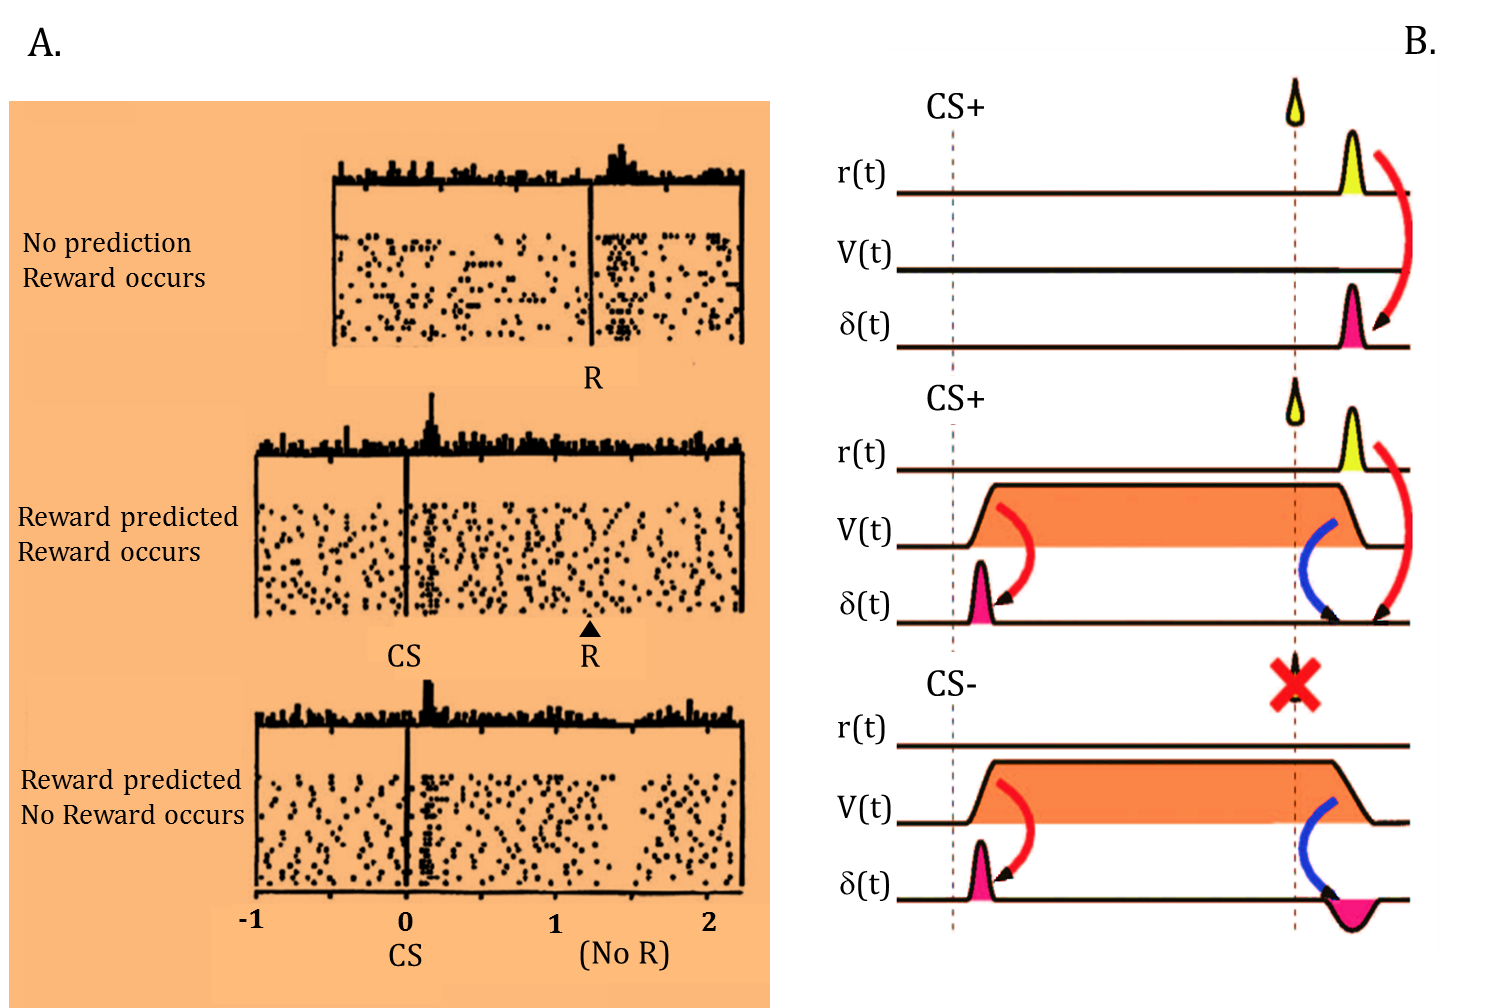
\includegraphics[scale=0.35]{figures/RewardDoyaRLSUM.png}
    \caption{Adapted from \cite{Doya}. In panel A: \textbf{Top two panels:} response associated to rewarded trials. \textbf{Lower panel:} response associated to unrewarded trials. In panel B: scheme of prediction error computing. \textbf{Top:} no prediction, reward occurs, the prediction error is positive. \textbf{Middle:} the reward occurs as expected, the prediction error is equal to zero. \textbf{Bottom:} the reward was predicted but did not occur.}
    \label{fig:RewDoyaSum}
\end{figure}
Based on broad knowledge on reward prediction signals, I assume that if the assembly-pairs activity codes for the reward prediction I can expect intense activity in the CS+ window when the animal learnt the task and was able to predict the reward (see figure \ref{fig:RewDoyaSum} A. middle); whereas I can expect little assembly-pair activation in CS+ window when the animal was uncertain to get the reward (see figure \ref{fig:RewDoyaSum} A. top), namely at beginning of the task. In other words I expected the assembly-pair activity in CS window to anti-correlate with the uncertainty to get the reward $\alpha_L(t)$, that I will call $\alpha(t)$ for ease from now on. Indeed, the uncertainty is high at the beginning of the task and goes down at the end of the original phase, to rise again at the beginning of the reversal phase. 
\begin{figure}
    \centering
 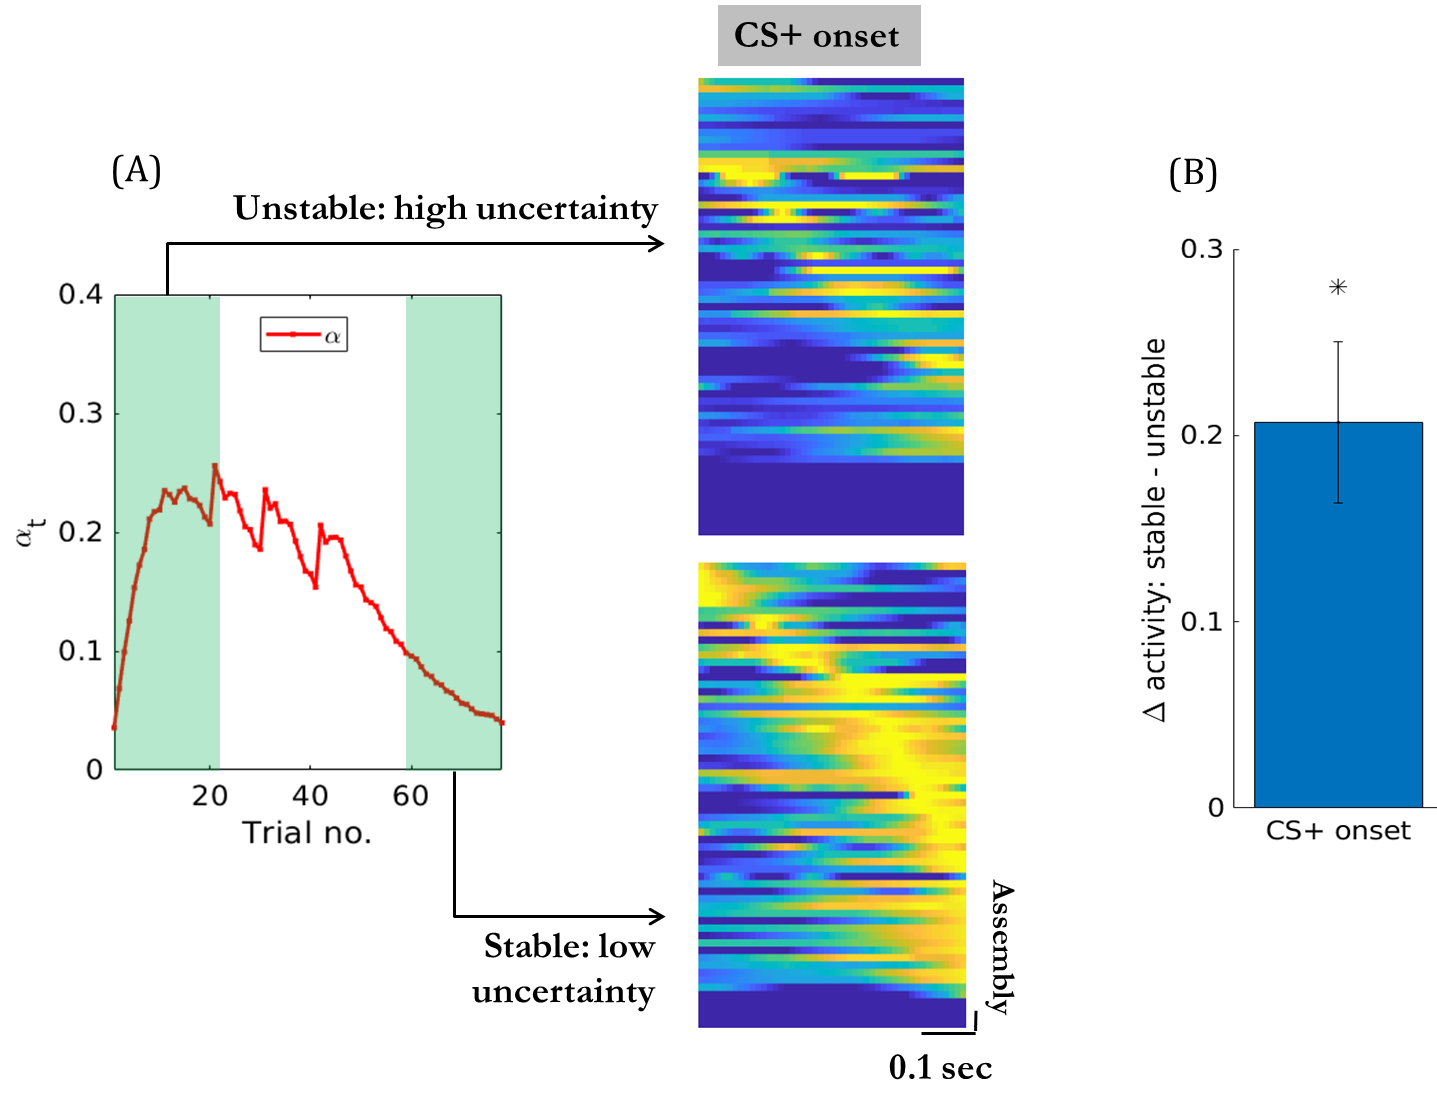
\includegraphics[scale=0.49]{figures/PreRegress.png}
 \caption{(A) Comparison between the uncertainty $\alpha(t)$ and the SPN-DAN assembly pairs activity in the stable and unstable phase. For this example only trials in which the rewarded odor was presented are shown. The analysis was restricted to the CS+ window, because the prediction of the reward happens immediately after the stimulus onset. If assembly pairs code for reward prediction, in the unstable phase characterized by high uncertainty to get the reward the assembly-pairs activity in CS+ window is low, whereas in the stable phase characterized by low uncertainty the assembly-pairs activity is high. The difference between the assembly-pairs activity in stable and unstable phase is significantly different to zero (B).}
\label{fig:StableUnstableAlphaCS}
\end{figure}
In figure \ref{fig:StableUnstableAlphaCS} I show an intuitive way to use the task variability in order to see the correlations with model functions. I divided the task in two phases: a first phase constituted by first trials in which the animal was learning the task and was uncertain about the reward outcome (I called this phase the $'$unstable$'$ phase); a second phase was constituted by last trials of the task in which the animal has learnt the task rule and it was more certain about the reward outcome when a rewarded or unrewarded odor is presented ($'$stable$'$ phase).\\I compared the assembly-pairs activity in unstable and stable phase. The difference between the two phases was significantly different from zero only for SPN-DAN pairs.\\This finding highlighted a possible specificity of assembly-pairs types coding, that will be proved in the next sessions.\\With similar arguments I can assume that, if the assembly-pairs compute reward prediction error their activity should correlate with the prediction error $\delta(t)$ in the US window. At the beginning of the task, when the prediction error is high I expect in the US window a high assembly-pairs response in conformity with the high surprise of the animal to get the reward, while when the task is learnt the surprise to get the reward and the prediction error are smaller and I expect less activity.\\In the next session I mathematically formalize these concepts in order to quantify the correlations with $\alpha(t)$ and $\delta(t)$; and hence test whether there is a specific VS-VTA interaction path involved in the reward prediction coding and prediction error computing. 
\section{Regression}
\label{sec:Regression}
In the previous sessions, I presented the Q Learning-Forgetting model to parameterize the learning functions. The main questions are: do assembly-pairs predict the reward and compute prediction error? Do different assembly-pair types compute different component of prediction error? More specifically, which assembly-pair types compute the evaluation component of the prediction error parameterized in the reinforcement learning model? As discussed in the previous session, if an assembly-pair computes reward prediction error I expect the assembly-activity being anti-correlated with the uncertainty $\alpha(t)$ in the CS window and correlated with the prediction error $\delta(t)$ in the US (real or expected reward) window. In order to quantify these correlations I regressed the assembly-pair activity on $\alpha (t)$ and $\delta (t)$. The two regressions were built separately: I regressed the assembly-pairs activity on the uncertainty $\alpha(t)$ in the CS window and on the prediction error $\delta(t)$ in the US (real or expected) window.\\Since the majority of the inter-regional pairs followed a Poisson distribution (see figure \ref{fig:DistributionEx}), I selected these pairs and built two generalized linear models with logarithmic link function, tailored for Poisson distributed data.
The assembly-pairs activity is a sample of n observations $\mathbf{Y}=(y_1, y_2,..., y_n)$ which can be treated as realizations of independent Poisson random variables, with $Y\sim P(\mu)$, in generalized linear model the mean (and therefore the variance), $\mu$, of the distribution depends on the independent variables, $X$, through:
$E (\mathbf {Y} )={\boldsymbol {\mu }}=g^{-1}(\mathbf {X} {\boldsymbol {\beta }})$ where $g$ is the link function, logarithmic in this case, $\boldsymbol{\beta}$ are unknown parameters estimated by the model, through which is quantified the relationship between the dependent and independent variables. The two regression models used can be written as follow:
\begin{equation}
    \log(\mu_t)=\beta_0+\beta\cdot\alpha(t-1)
    \label{eq:regrAlpha}
\end{equation}
one can notice that in equation \ref{eq:Qlearning} the uncertainty of the trial $t$ ($\alpha(t)$) is used to update the reward expectation value of the trial $t+1$ ($Q_{s,a}(t+1)$), the uncertainty $\alpha(t)$ updated only after the update of $\delta(t)$, which happens at the reward time, then in the CS window of the trial $t$, where the update is not yet computed, I regress the assembly-pair activity of the trial $t$ on the uncertainty $\alpha(t-1)$.
\begin{equation}
    \log(\mu_t)=\beta_0+\beta\cdot\delta(t)
    \label{eq:regrDelta}
\end{equation}
On the other hand I regressed the assembly-pair activity on the prediction error $\delta$ in US the window, which started either at the reward time or at the expected reward time when the unrewarded odor was presented (see \hyperref[sec:TaskResp]{~Chapter \ref*{sec:TaskResp}} for the window specification). In this window the update is already computed, thus I regressed assembly activity at the trial $t$ on the prediction error of the trial $t$.\\
Before discussing the results a clarification about the meaning of the coefficient $\beta$ in Poisson regression is needed.\\
Coefficient $\beta$ tells us how changes in the independent variables are associated with changes in the dependent variable.
The two regression presented can be written as Poisson regression with one independent variable $x$:
\begin{equation}
    \log(\mu)=\beta_0+\beta_1\cdot x
    \label{eq:betaCoeff}
\end{equation}
So, if I have an initial value of the covariate $x_0$, then the predicted value of the mean $\mu_0$ is given by:
\begin{equation*}
    \log(\mu_0)=\beta_0+\beta_1\cdot x_0
    \label{eq:betaCoeff0}
\end{equation*}
If I now increase the covariate by 1, I get a new mean $\mu_1$,
\begin{equation*}
    \log(\mu_1)=\beta_0+\beta(x_0+1)=\beta_0+\beta_1x_0+\beta_1=\log(\mu_0)+\beta_1
    \label{eq:betaCoeff1}
\end{equation*}
So the log of the mean of $Y$ increases by $\beta_1$ when $x$ is increased by 1.
In general one can say that in Poisson regression, the regression coefficients $\beta$ are interpreted as the difference between the log of expected counts, where formally, this can be written as:
\begin{equation}
    \beta=\log(\mu_{t+1})-\log(\mu_t)
    \label{eq:BetaRelLog}
\end{equation}
One is in general not primarily interested in how the log mean changes and want to know on average how $Y$ changes. Therefore I performed an exponential transformation:
\begin{equation}
    \mu_{t+1}=\mu_t\cdot \exp(\beta)
    \label{eq:BetaRelExp}
\end{equation}
It is important to note the difference with the linear regression: in normal linear regression the relationship between the observations and $\beta$ is additive, whereas in Poisson linear regression the relationship is multiplicative.\\The equation \ref{eq:BetaRelExp} can be written in term of the percentage increase of the count number after dividing both members of the equation by $\mu_t$ and subtracting both members by 1, doing so I obtain:
\begin{equation}
\exp(\beta)-1=\frac{\mu_{t+1}-\mu_t}{\mu_t}
    \label{eq:BetaPerc}
\end{equation}
The last equation can be interpreted as the percentage increase of the count number.\\This interpretation allowed us to use the coefficients $\beta$ in order to understand how changes in percentage the assembly activity in relation to the change of the variables $\alpha$ and $\delta$.\\Since I compared results among different assembly-pairs and sessions, I needed to standardize the coefficients $\beta$ resulting from the regression. Standardized $\beta$ can be expressed through the following:
\begin{equation}
    \beta^*=\beta\cdot\frac{\sigma(x)}{\sigma(Y)}
    \label{eq:betaStand}
\end{equation}
where $\sigma(x)$ ($\sigma(Y)$) is the standard deviation of x (Y).
Results of two regressions are reported in figure \ref{fig:AlphaDeltaReg}.\\
To easily read the plot in the term of percentage instead of the $\beta$ coefficients, I reported the $\beta^*$ transformed as:
\begin{equation}
    \beta^*\rightarrow \exp(\beta^*)-1
    \label{eq:BetaPlot}
\end{equation}
\begin{figure}[H]
    \centering
    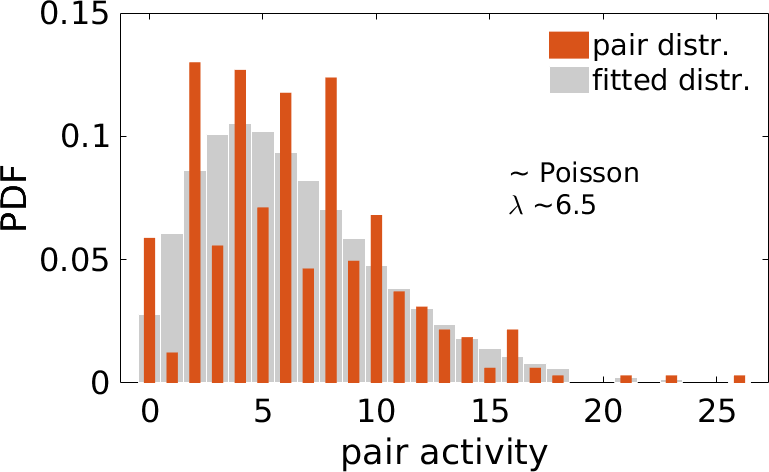
\includegraphics[scale=0.25]{figures/Rev2An2As1_rew.png}
    \hspace{1cm}
    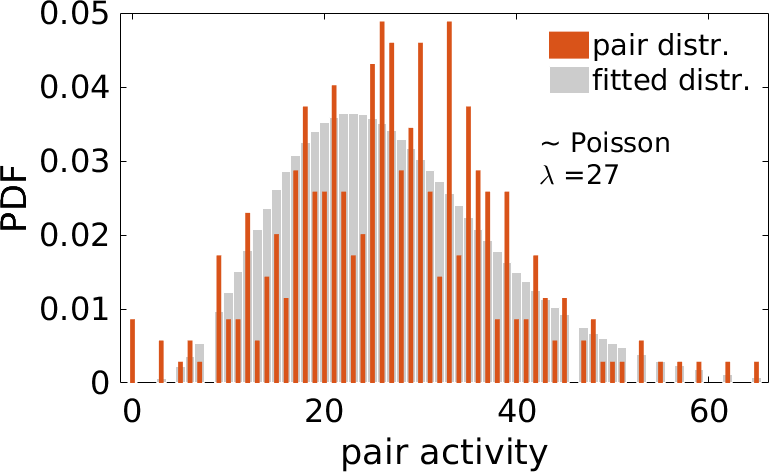
\includegraphics[scale=0.25]{figures/Rev2An2As2.png}
    
    \vspace{1cm}
    
    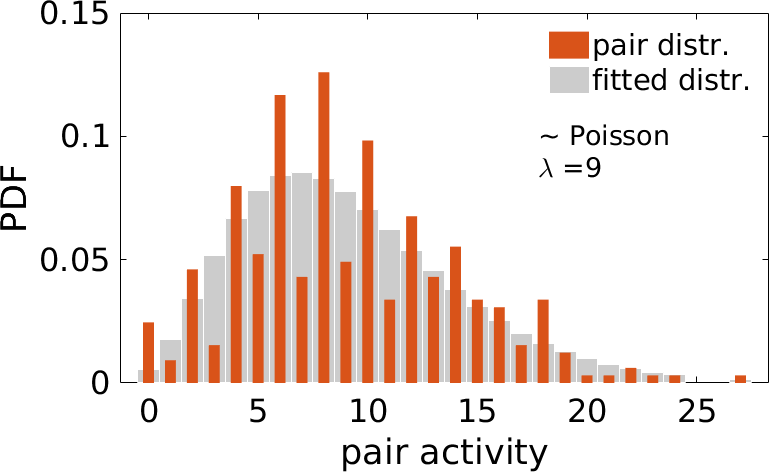
\includegraphics[scale=0.25]{figures/Rev2An2As1.png}
    \hspace{1cm}
    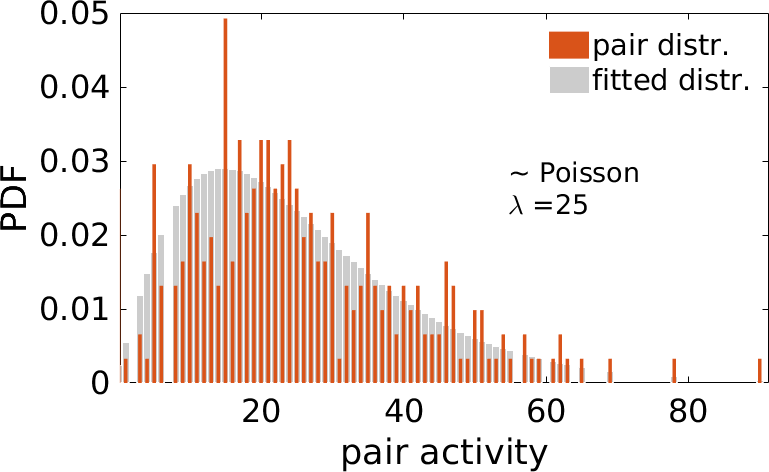
\includegraphics[scale=0.25]{figures/Firstrev1An4As5.png}
    \caption{Some example of pair activity distributions in CS and US window. Assembly-pair distribution can be approximated with Poisson's distribution. To regress the assembly-pair activity on $\alpha(t)$ and $\delta(t)$, I used a Poisson linear model which is tailored for Poisson distributed observations.}
    \label{fig:DistributionEx}
\end{figure}
I reported only the statistically significant coefficients. After the pruning of only Poisson distributed assembly-pairs, and considering only statistically significant associations between the response and the regressor, I had in total the $33\%$ of SPN-DAN assembly-pairs when I regressed the activity on $\alpha$ and the $25\%$ of SPN-DAN assembly-pairs after regressing the activity on $\delta$.\\In figure \ref{fig:AlphaDeltaReg} the $\beta^*$ coefficients as defined above resulting from regression using the model with $\alpha$ as regressor defined in equation \ref{eq:regrAlpha} (figure \ref{fig:AlphaDeltaReg} top left) and from regression using the model with $\delta$ as regressor defined in equation \ref{eq:regrDelta} (figure \ref{fig:AlphaDeltaReg} bottom left). $\beta^*$ above zero indicated a positive correlation between the assembly-pair activity and the model variable $\alpha$ ($\delta$) whereas a $\beta^*$ below zero indicated a negative correlation. The value of $\beta^*$ indicated the change in percentage in assembly activity in relation to a change of one unit of the variable $\alpha$ ($\delta$). On the right side of the plots the empirical cumulative distribution function (ECDF) of $\beta^*$ related to the regression with $\alpha$ (top right) and with $\delta$ (bottom right). In purple SPN-DAN assembly-pairs, in dark green FSN-DAN assembly-pairs. The sign of correlation between assembly-pairs and regressors was extremely clear when I looked at ECDF of $\beta^*$: for SPN-DAN pairs in case of regression on $\alpha$, ECDF was asymmetric in favour of negative $\beta^*$, whereas it was symmetrical distributed for FSN-DAN pairs. On the other hand the asymmetry of ECDF for SPN-DAN pairs was inverted when I regressed $\delta$, whereas it remained approximately symmetric for FSN-DAN pairs.
\begin{figure}[H]
    \centering
    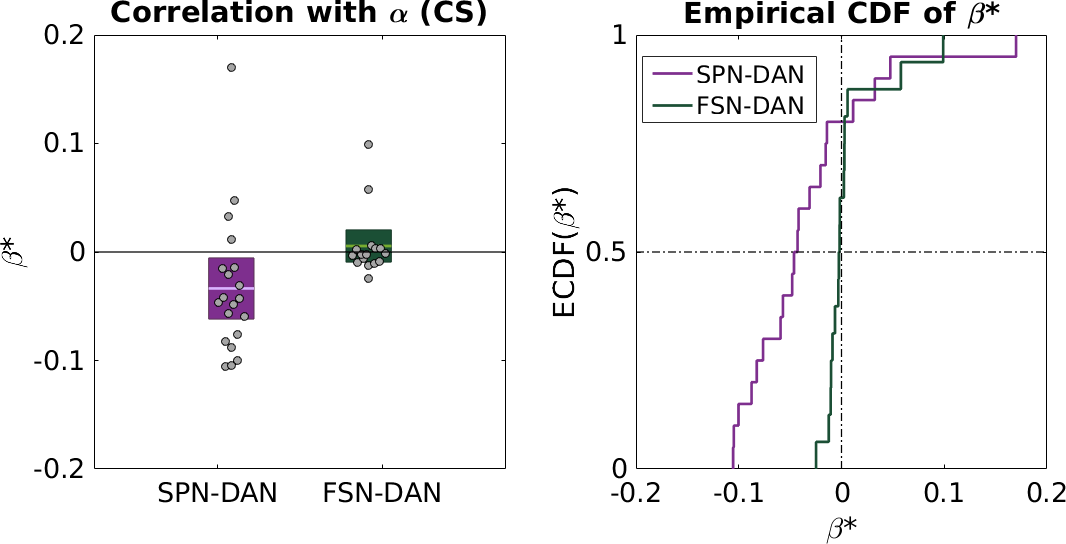
\includegraphics[scale=0.42]{figures/alphaRegrNew3.png}
    
    \vspace{1cm}
    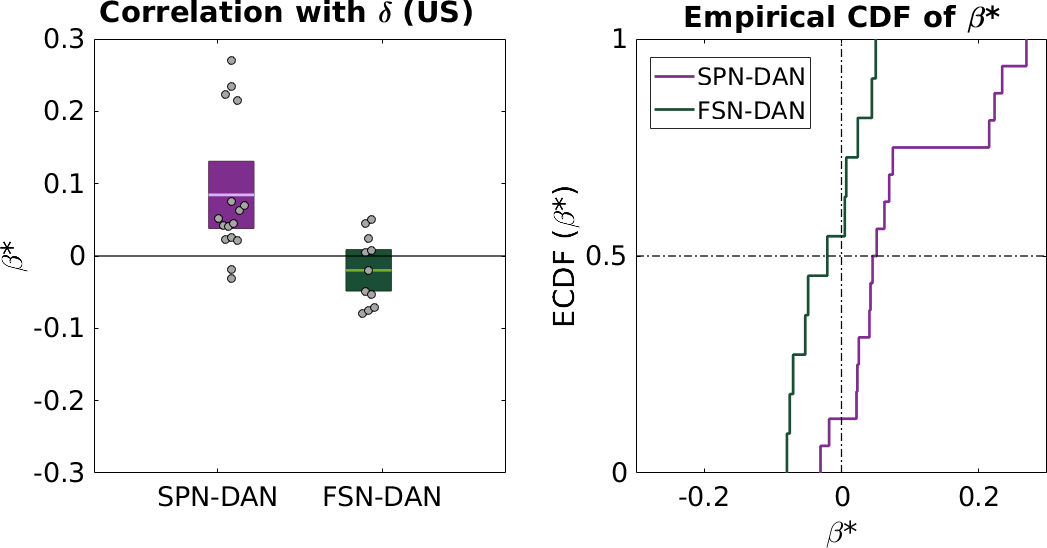
\includegraphics[scale=0.42]{figures/deltaRegr3.png}
    \caption{\textbf{Top:} Results obtained regressing $\alpha$. \textbf{Bottom:} Results obtained regressing $\delta$. \textbf{Left:} Box plot of standardized $\beta^*$ regression coefficients. In Poisson linear model the coefficient $\beta$ indicate the variation in percentage of the observations values when the dependent variable increase of one unit. Since $\beta^*$ were approximately normally distributed, I plotted the $\beta^*$ in such a way that points in box plot were layed over a $1.96$ SEM ($95\%$ confidence interval) in the coloured box. Row data are jittered along x-axis for clarity. \textbf{Right:} empirical cumulative distribution function of $\beta^*$}
    \label{fig:AlphaDeltaReg}
\end{figure}
To further assess whether both $\alpha$ and $\delta$ were represented in different ways in SPN-DAN and FSN-DAN pairs I conducted two Mann-Withney-U tests on the regression coefficients, from which resulted that in both cases $\beta^*$ were differently distributed in SPN-DAN and FSN-DAN pairs ($p-value=0.017$ for $\beta^*_{\alpha}$ and $p-value=0.016$ for $\beta^*_{\delta}$). Furthermore I compared the distributions of $\beta^*_{\alpha}$ and $\beta^*_{\delta}$ between each other only in SPN-DAN pairs: these coefficients were not equally distributed ($p-value=4.92\times10^{-5}$). I concluded that SPN-DAN assembly-pairs anti-correlate with the uncertainty $\alpha$ in CS window and correlate with prediction error $\delta$ in US window. On the other hand FSN-DAN did not show any preferential direction in correlation with $\alpha$ and $\delta$ and the $\beta^*$ were equally distributed around zero.\\These results confirmed the hypothesis that SPN-DAN pairs specifically convey the reward prediction error signal.
\section{Conclusion}
\label{sec:concRL}
Based on a starting hypothesis on the specific role of different interregional assembly-pair types in reward prediction error coding (see \hyperref[sec:TaskResp]{~Chapter \ref*{sec:TaskResp}}), I parameterized the learning functions through a reinforcement learning model, in order to establish a mathematical relationship between the assembly-pair activity and the functions mimicking the reward prediction signal.\\The reward prediction error is defined in reinforcement learning model theory as the difference from the expected reward value, which evolves in the model according to a defined learning dynamic, and the received outcome. As discussed in \hyperref[sec:TaskResp]{~Chapter \ref*{sec:TaskResp}} this component of prediction error signal is the main component, involved in the effective valuation of the signal, which follows an initial detection of the stimulus.\\I set up four models and assessed the best model with Likelihood ratio test when the models to compare were nested, and with the Bayesian Information Criterion when the models compared had same number of parameters. The winner model was a learning-forgetting model with dynamical learning rate, that mimics the uncertainty of the animal to get the reward. This variable $\alpha$ is equally important as the reward prediction error $\delta$ in prediction error coding.\\The hypothesis, based on task related response of assembly-pair types and on the length of average inter-units lag distribution, was that SPN-DAN pairs are involved in main component of prediction error signal, parameterized by the model. On the other side, FSN-DAN pairs could be involved only in the detection component of prediction error signal because of their early and diversified activation. Those pairs unspecifically responded to the stimulus or other events, such us the choice; their activity is involved in non-trivial emotional coding.\\These hypotheses bear the idea of an highly specificity in information transfer in the circuit.\\To mathematically formalize this concept, I expected that SPN-DAN pairs anti-correlate with the uncertainty $\alpha$ in the stimulus window, being $\alpha$ the variable mimicking the uncertainty, and being the prediction error signal more strong at the stimulus presentation as the certainty to get the reward increases. On the other hand, if it was true that the prediction error signal is formed in SPN-DAN interactions, I expected as well SPN-DAN pairs to correlate with the prediction error $\delta$ at the retrieval.\\I modeled two linear Poisson regression models and I regressed assembly-pair activity on the uncertainty $\alpha$ and the prediction error $\delta$. Figure \ref{fig:AlphaDeltaReg} shows on the left side the box-plots of resulting regression parameters when I regress the activity on $\alpha$ (top left) and $\delta$ (bottom left). On the right side of figure \ref{fig:AlphaDeltaReg} the empirical distribution function corresponding to $\beta^*$ shown on the left.\\
The resulting regression coefficients showed, as predicted, that SPN-DAN pairs negatively correlated with the uncertainty and positively correlated with the prediction error, conversely FSN-DAN pairs did not show any significant correlation either with the uncertainty or the prediction error.\\These results reveal that the evaluation component of prediction error signal was formed through the SPN-DAN interactions. 
